\chapter{FAT 32}
\label{cap:Fat}
    Nel presente capitlo introduciamo alcuni concetti generali riguardanti il file system FAT. 
    Successivamente procederemo con un maggior dettaglio analizzando le varie strutture di cui è composto e le procedure mediante le quali i dati vengono salvati e prelevati dal disco. 
  \section{Carateritiche}
  \label{sec:Carateristiche}
    La File Allocation Table, in sigla FAT, è un file system sviluppato inizialmente da Bill Gates e Marc McDonald. È il file system primario per diversi sistemi operativi DOS e Microsoft Windows fino alla versione Windows ME.\\
    La FAT è relativamente semplice ed è supportata da moltissimi sistemi operativi. Queste caratteristiche la rendono adatta ad esempio per i Floppy Disk e le Memory Card e può anche essere utilizzata per condividere dati tra due sistemi operativi diversi.\\
    Il più grande problema del File System FAT è la \textbf{frammentazione}. Quando i file vengono eliminati, creati o spostati, le loro varie parti si disperdono sull'unità, rallentandone progressivamente la lettura e la scrittura. Una soluzione a questo inconveniente è la deframmentazione, un processo che riordina i file sull'unità. Questa può durare anche diverse ore e deve essere eseguita regolarmente per mantenere le prestazioni dell'unità.\\
    Esistono varie versioni di questo file system, in questa sede analizziamo soltanto il FAT32. \\ 
    Il FAT32 presenta alcuni limiti, si possono gestire volumi che hanno una grandezza compresa tra i 512MB e 32 GB, questi limiti sono imposti dalle routine Microsoft, infatti esistono routine di terze parti che permettono di superare questi limiti. \\
    Il file system FAT possiede anche un limite sulla grandezza massima dei file che non può eccedere i 4GB. \\

   \section{Struttura}
       Il File system FAT usa un criterio di allocazione dei dati basato sull'utilizzo di liste concatenate. Per poter rintracciare queste liste, vengono salvate nella FAT presente sul disco. 
	Grazie all'utilizzo della tabella FAT viene anche risolto il problema della gestione dello spazio libero. Il funzionamento della FAT è ampiamente spiegato nel paragrafo \ref{GestioneFat}.\\
      La struttura generale di un volume FAT32 è composta da tre regioni principali: 
        \begin{enumerate}
           \item  \textbf{Regione riservata} Regione nella quale troviamo tutte le informazioni di basso livello attinenti al volume
           \item  \textbf{Regione FAT}  Regione nella quale è presente la tabella FAT indispensabile per la gestione dei dati sul disco. 
           \item  \textbf{Regione Data} Regione nella quale sono presenti i dati veri e propri.
         \end{enumerate}
    
    \begin{figure}[h]
    \centering
    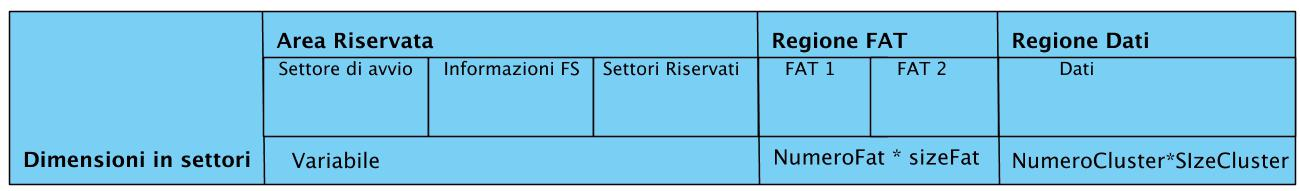
\includegraphics[width=350px,height=70px]{./Immagini/struttura.jpg}
     % struttura.jpg: 1300x191 pixel, 96dpi, 34.40x5.05 cm, bb=0 0 975 143
    \caption{Struttura Volume FAT}
    \label{Fig.: Struttura Volume FAT32}
    \end{figure}

    \subsection{Regione Riservata}

            La regione riservata è la prima regione che troviamo nel volume e contiene tutte le informazioni di basso livello necessarie per un corretto funzionamento del file system stesso. A sua volta questa regione è suddivisa in zone diverse. 
            \begin{itemize}
             \item \textbf{Boot Sector} Questa è la prima struttura presente in un volume FAT, occupa il primo settore del volume  (settore zero) ed è la più importante della regione riservata.\\
	      Il Boot sector include un'area chiamata \textbf{BIOS Parameter Block (BPB)} che contiene alcune informazioni base per il funzionamento del file system quali ad esempio tipo del file system e posizione delle altre regioni nel disco. Il BPB occupa i byte dall'offset 0x1B fino all'offset 0x34 del Boot Sector. \\
	      Oltre al BPB nel boot sector troviamo anche il codice del boot loader necessario per avviare un sistema operativo.
	     La successiva tabella rappresenta schematicamente la struttura del boot sector di un volume FAT32 :
	  
		      \begin{center}
		      \begin{tabular}{|r|r|l|}\hline
			  \textbf {Offset} & \textbf{Lunghezza} & \textbf{Descrizione}\\\hline
			  0x00 & 3 & Salta istruzione\\\hline
			  0x03 & 8 & Nome	\\\hline
			  0x0B & 2 & Estensione\\\hline
			  0x0D & 1 & Bytes per settore \\\hline
			  0x0E & 2 & Numero dei settori di riserva\\\hline
			  0x10 & 1 & Numero di tabelle FAT \\\hline
			  0x11 & 2 & FAT32 vale 0 \\\hline
			  0x13 & 2 & Settori totali. \\\hline
			  0x15 & 1 & Tipo di descrittore. \\\hline
			  0x16 & 2 & Settori per FAT (per FAT12/16) \\\hline
			  0x18 & 2 & Settori per traccia \\\hline
			  0x1A & 2 & Numero di testine \\\hline
			  0x1C & 4 & Settori nascosti \\\hline
			  0x20 & 4 & Totale settori. \\\hline
			  0x24 & 4 & Settori occupati da una FAT \\\hline
			  0x28 & 2 & FAT flags \\\hline
			  0x2A & 2 & Versione \\\hline
			  0x2C & 4 & Cluster Root Directory \\\hline
			  0x30 & 2 & Numero settore FS Information \\\hline
			  0x32 & 2 & Numero settore di Backup \\\hline
			  0x34 & 12 & Riservato \\\hline
			  0x40 & 1 & Numero Driver \\\hline
			  0x41 & 1 & Riservato \\\hline
			  0x42 & 1 & Firma estesa \\\hline
			  0x43 & 4 & ID \\\hline
			  0x47 & 11 & Volume Label \\\hline
			  0x52 & 8 & FAT File sytem type\\\hline
			  0x5A & 420 & Codice Boot loader\\\hline
			  0x1FE & 2 & Firma boot sector\\\hline
		      \end{tabular}
		      \end{center}



	     \end{itemize}
     
	  

	     \begin{itemize}
	     \item \textbf{Fat Information Sector}
	  
	      Introdotto con la FAT32 per accelerare i tempi di accesso di alcune operazioni (i.e. la quantità di spazio libero), occupa generalmente il settore 1, nel record di avvio 0x30. Ha dimensione pari a 512 byte. Contiene un campo nel quale è specificato lo spazio libero rimanente ( offset 0x1E8 ) e il primo cluster dal quale iniziare la ricerca del cluster libero (oofset 0x1F0).
	      \newpage
	      La tabella successiva riepiloga i vari campi :
		      \begin{center}
		      \begin{tabular}{|r|r|l|}\hline
			  \textbf {Offset} & \textbf{Lunghezza} & \textbf{Descrizione}\\\hline
			  0x00  & 4  & Firma File System Info\\\hline
			  0x04  & 480&Riservati	\\\hline
			  0x1E4 & 4  & Firma File System Info\\\hline
			  0x1E8 & 4  & Numero cluster liberi \\\hline
			  0x1EC & 4  &  Cluster dal quale iniziare la ricerca \\\hline
			  0x1F0 & 14 &  Riservato \\\hline
			  0x1FE & 2  &  Firma File System Info \\\hline
		      \end{tabular}
		      \end{center}
 	    \end{itemize}
	  

	    \begin{itemize}
	       \item \textbf{Settori Riservati}
	      Alcuni settori riservati, sono a disposizione per essere usati per rimpiazzare i settori che sono danneggiati nel disco. 
	    \end{itemize}

    \subsection{Regione Fat}
	\label{sec:RegioneFat}
	      La regione FAT è la regione del disco nella quale sono salvate la tabelle FAT. Per avere una maggior sicurezza nel salvataggio dei dati sono presenti per default due tabelle FAT. Il numero di tabelle 
	      presenti nel disco e contenuto nel boot sector ed è configurabile in fase di formattazione.
    \subsection{Regione Dati}
	      La regione Dati è la regione che inizia successivamente alla regione FAT ed è quella nelle quali sono presenti i veri propri dati. 
	      Questa regione è vista dal file system come suddivisa in un certo numero di blocchi di grandezza uguale. Anche in questo caso tutte le informazioni necessarie per la gestione dei blocchi e più in generale della zona dati sono presenti nel Boot sector.
    \section{Getione Fat}
    \label{GestioneFat}
        Dopo aver presentato la struttura generale di un volume FAT 32, analizziamo il meccanismo con il quale vengono salvati i dati. 
	Una partizione è suddivisa in \textbf{cluster} di egual grandezza. I cluster sono dei blocchi di spazio continuo, la cui grandezza dipende dal tipo di file system e dalla grandezza della partizione. 
       Tipicamente la grandezza di un cluster oscilla tra i 2kB e 32 kb ed è stabilita in fase di formattazione.\\
        Ogni file può occupare uno o più cluster in base alla sua grandezza, quindi il file viene rappresentato da una catena di cluster. Le catene sono realizzate mediante una lista concatenata semplice.
        L'insieme dei cluster di cui è composto un file non necessariamente vengono salvati in posizioni adiacenti, ciò comporta una dispersione dei cluster per tutto il disco con un degrado delle prestazioni. 
	Questo fenomeno prende il nome di \textbf{frammentazione}.\\
	La tabella Fat è composta da entry a 32 bit ed posizionata nella regione FAT ( vedi § \ref{sec:RegioneFat} ). Lo scopo di tale tabella è quello di mappare tutti i cluster di cui è composto un volume con la relativa entry. 
	Ogni entry può assumere i seguenti valori : 

	  \begin{itemize}
	   \item Il numero del cluster successivo.
	  \end{itemize}

	  \begin{itemize}
	   \item Il valore speciale di fine catena (EOC)
	  \end{itemize}

	  \begin{itemize}
	   \item Il valore speciale che segnala il cluster come riservato
	  \end{itemize}

	   \begin{itemize}
	    \item  Il valore speciale che segnala il cluster come mal funzionante
	  \end{itemize}

	  \begin{itemize}
	   \item Zero che identifica il cluster come libero
	  \end{itemize}
    
    Usando questa tecnica si crea una corrispondenza univoca tra i cluster del disco e le entry della tabella Fat. Per esempio, se si volesse sapere lo stato del cluster 42 è sufficiente analizzare l'entry numero 42 della tabella. \\
    La struttura della FAT è molto semplice, e di conseguenza anche le operazioni per la gestione dei file risultano essere semplificate.\\
    Infatti per ricercare un cluster libero si scorre la tabella finché non si trova un cluster marcato come libero.
    Per rintracciare tutti i cluster di cui è formato un file è sufficiente conoscere il primo cluster della catena.
    Utilizzando il numero del primo cluter come indice nella tabella si può risalire al cluster successivo, se presente, poiché il suo valore è contenuto nell'entry letta. Usando il valore presente nella nuova entry si può proseguire nella ricerca dei cluster usando la stessa procedura.\\
    La ricerca terminerà quando nell'entry della tabella è presente il valore EOC.
    Le  prime due entry nella FAT contengono speciali valori. La prima entry contiene una copia del media Descriptor ( Descrive il device, contenuto nel boot sector, offset 0x15). I rimanenti bit vengono settati ad 1.\\ 
    La seconda entry contiene il valore di \textit{End Of Chain}, cioè il valore usato per indicare la terminazione di una catena di cluster. I due Bit più significativi di questa entry sono usati per identificare lo stato di occupato del disco e rilevare possibile errori di montaggio.\\ 
    Poiché le prime due entry sono riservate il primo cluster utile della tabella FAT, risulta essere il 2. Il cluster 2 tipicamente è il primo cluster della catena che rappresenta la root directory. \\
    La tabella successiva riassume i valori che possono assumere le entry FAT e il loro significato.\\

    \begin{center}
\begin{tabular}{|c|c|}\hline
\textbf {FAT32} & \textbf{Descrizione}\\\hline
0x00000000 & Cluster Libero\\\hline
0x00000001 & Riservato\\\hline
0x00000002-0x0FFFFFEF & Cluster usabili\\\hline
0x0FFFFFF0-0x0FFFFFF6 & Riservati\\\hline
0xFFFFFF7 & Bad Cluster\\\hline
0x0FFFFFF8-0xFFFFFFFF & End Of Chain\\\hline
    \end{tabular}
    \end{center}

Come si può notare dai Valori della tabella il FAT32 utilizza solamente 28 bit per indicizzare le varie entry della tabella FAT, solitamente i 4 bit più significativi sono settati a zero, ma essendo riservati il loro valore non deve essere modificato. 

    \section{Gestione Directory}
    \label{gest:dir}
Una \textbf{tabella directory} è un file speciale che che rappresenta una cartella.
Ogni riga di questa tabella prende il nome di \textbf{entry} e viene associato ad un file.  Un \textbf{entry} è una struttura dati formata da 32 byte, che contiene le informazioni necessarie per la gestione dei file. 
Sono state introdotte nel FAT32 due tipi di entry diverse. \\
Il primo tipo, presente sin dalla prima versioni del FAT 32 ha lo scopo di contenere le informazioni necessarie per la gestione dei file. La tabella successiva rappresenta tale entry : 

\begin{center}
\begin{tabular}{|l|c|l|}\hline
\textbf{Offset} & \textbf{Lunghezza} & \textbf{Descrizione}\\\hline
0x00 & 8 & Nome file\\\hline
0x08 & 3 & Estensione File\\\hline
0x0B & 1 & Attributi\\\hline
0x0C & 1 & Riservato\\\hline
0x0D & 1 & Tempo creazione ms\\\hline
0x0E & 2 & Tempo creazione\\\hline
0x10 & 2 & Data di creazione\\\hline
0x12 & 2 & Data Ultimo accesso\\\hline
0x14 & 2 & 2 byte piu significativi indirizzo cluster\\\hline
0x16 & 2 & Tempo Ultimo Modifica\\\hline
0x18 & 2 & Data ultimo modifica\\\hline
0x1A & 2 & 2 byte meno significativi cluster\\\hline
0x1C & 4 & Grandezza file\\\hline
\end{tabular}
\end{center}

I campi principali sono il nome, formato da 8 caratteri più 3 caratteri di estensione, entrambi codificati secondo il set di caratteri OEM. 
L'insieme di questi due campi d'ora in poi verrà riferito con il termine nome corto. \\
Il nome corto del file viene generato mediante un algoritmo fornito dalla Microsoft stessa, il quale si occupa di risolvere le problematiche che nascono nel caso in cui siano presenti nomi simili\footnote{Per il concetto di Nomi simili si intendono nomi uguali per i primi 8 caratteri.}, nella stessa cartella.\\
Le altre due informazioni principali presenti in questa struttura sono il numero del primo cluster, necessario per risalire alla catena di cui è composto un file e la grandezza del file, necessaria per 
eseguire le operazioni di scrittura e lettura in maniera corretta. 
Sin dalla prima versione, la lunghezza del nome del file a soli 11 caratteri è stato un limite.\\
Per superare questo limite si è deciso di introdurre delle entry il cui unico scopo era quello di estendere il nome dei file. Questo tipo di entry è riassunta nella successiva tabella.   

\begin{center}
\begin{tabular}{|l|c|l|}\hline
\textbf{Offset} & \textbf{Lunghezza} & \textbf{Descrizione}\\\hline
0x00 & 1  & Indice\\\hline
0x01 & 10 & Nome1\\\hline
0x0B & 1  & Attributi\\\hline
0x0C & 1  & Tipo\\\hline
0x0D & 1  & Checksum\\\hline
0x0E & 12 & Nome2\\\hline
0x1B & 2  & Riservato\\\hline
0x1D & 4  & Nome3\\\hline
\end{tabular}
\end{center}

Queste entry occupano le posizioni che precedono la entry con le informazioni per la gestione dei file. Il nome inserito in questo tipo di entry d'ora in avanti verrà identificato con il termine nome lungo.
Per essere sicuri di associare il nome lungo alla giusta entry, è presente il campo checksum che costituisce il risultato della funzione checksum fornita dalla Microsoft calcolata sul nome corto. 
Per poter risalire a tutte le entry che formano il nome lungo è sufficiente seguire l'indice presente nella prima posizione, finché non si raggiunge l'ultima entry identificata da un marcatore di fine lista.
Con questa soluzione i nomi gestibili da un file system FAT32 possono raggiungere la lunghezza di 255 caratteri. 

\begin{figure}[h]
 \centering
 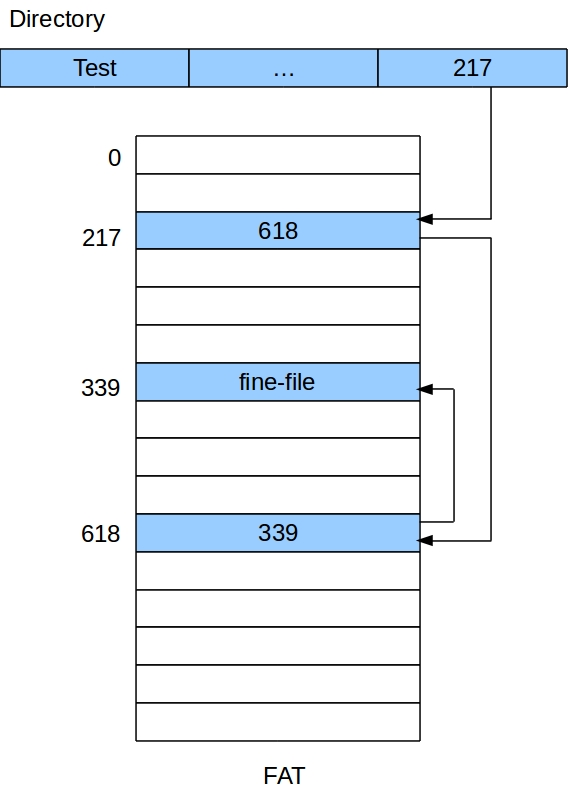
\includegraphics[width=250px,height=300px]{./Immagini/fat.jpg}
 % fat.jpg: 568x806 pixel, 72dpi, 20.04x28.43 cm, bb=0 0 568 806
 \caption{Esempio di una catena FAT}
 \label{Fig.:FAT}
\end{figure}


    \section{Differenze Specifiche}
     Non tutte le specifiche Microsoft esposte nei paragrafi precedenti sono state rispettate, o per aumentare l'efficienza del sistema generale o per avere delle semplificazioni realizzative. 
     La differenze con le specifiche Microsoft sono: 
    
     \begin{itemize}
    
     \item Le tabelle fat di backup vengono ignorate. Ho scelto di ignorare le tabelle di backup per una questione di efficienza, altrimenti ogni scrittura sulla  FAT primaria comporterebbe anche delle scritture 
     nelle FAT di backup che comprometterebbero le prestazioni. Per migliorare quest'aspetto si potrebbe inserire un meccanismo che ad intervalli regolari copia la FAT  primaria nelle FAT di backup.\\
 
     \item Il parametri presenti nel settore Fat Information Sector  la gestione delle zone libere del disco sono stati ignorati in quanto per semplificare e ottenere delle prestazioni migliori si è scelto di caricare l'intera FAT in memoria, quindi la ricerca di un cluster non comporta nessuna operazione sul disco.\\

     \item Ho ignorato i settori di backup del boot sector e in generale la gestione dei settori danneggiati per semplificare la gestione della FAT.\\

     \item Ho ignorato il problema della frammentazione. \\

       
     \end{itemize}
    \section{Conclusione}
    In questo capitolo è stata fatta un introduzione molto semplice al funzionamento del FAT, per eventuali approfondimenti fare riferimento alla documentazione microsoft. 
     Come si è potuto notare dalle spiegazioni dei capitoli precedenti il file system risulta essere molto facile da un punto di vista implementativo. 
      Se si analizzano le prestazioni e i limiti di questo file system      si nota che è poco scalabile e le prestazioni con grandi quantità di dati sono molto scarse, rendendolo quasi inutilizzabile. 
     Un modo per migliorare le prestazioni del file system è l'introduzione di un sistema di cache delle scritture / letture. Questa soluzione è quella adottata nella maggior parte dei sistemi operativi commerciali, 
     che grazie altra struttura modulare ( spiegata nel capitolo § \ref{cap:Struttutra_Progetto} ) posso essere introdotti anche qui. 
      
\clearpage{\pagestyle{empty}\cleardoublepage}

%%% Local Variables: 
%%% mode: latex
%%% TeX-master: "tesi"
%%% End: 